\newpage
\subsection{Address Resolution Protocol}
Lo scopo del protocollo ARP descritto in \cite{RFC0826} e in \cite{RFC5227} è quello di eseguire una mappatura tra indirizzo IP e indirizzo MAC di una macchina all'interno di una rete locale Ethernet.\\
La notazione seguente utilizzata nei pacchetti è ripresa da \cite{RFC0826}:
\begin{lstlisting}
    ar$hrd: Hardware address space 
    ar$pro: Protocol address space
    ar$hln: byte length of each hardware address
    ar$pln: byte length of each protocol address
    ar$op:  opcode (request | reply)
    ar$sha: Hardware address of sender 
    ar$spa: Protocol address of sender 
    ar$tha: Hardware address of target
    ar$tpa: Protocol address of target
\end{lstlisting}
In Figura \ref{fig:ARP} vediamo come si modella il protocollo ARP.\\
Una macchina, appena connessa alla rete o accesa, si mette subito in ascolto con l'oggetto ANNOUNCE\_WAIT e, allo stesso tempo, utilizza gli oggetti getIPAddress per generare un indirizzo IP sul quale essere contattata, getProtocolType e getMACAddress  per ricavare informazioni sul tipo di protocollo ethernet da utilizzare e l'indirizzo MAC della sua scheda di rete.\\
A questo punto utilizza queste informazioni per creare attraverso l'oggetto createProbePackage un pacchetto da inviare in broadcast a tutte le macchine della rete.\\
Successivamente attende un tempo predefinito attraverso l'oggetto PROBE\_WAIT, prima di spedire il pacchetto attraverso l'oggetto EthernetOUT e ritornare nello stato di ANNOUNCE\_WAIT.\\
Se nell'arco di un tempo predefinito non arriva nessun pacchetto dall'oggetto EthernetIN, procede con la conferma dell'indirizzo IP attraverso la creazione di un nuovo pacchetto con l'oggetto createAnnouncePackage, il quale verrà sempre spedito in broadcast attraverso l'oggetto EthernetOUT.\\
Se invece riceve un pacchetto dall'oggetto EthernetIN, ricomincia generando un nuovo indirizzo IP.\\
\begin{figure}[h!] 
    \centering 
    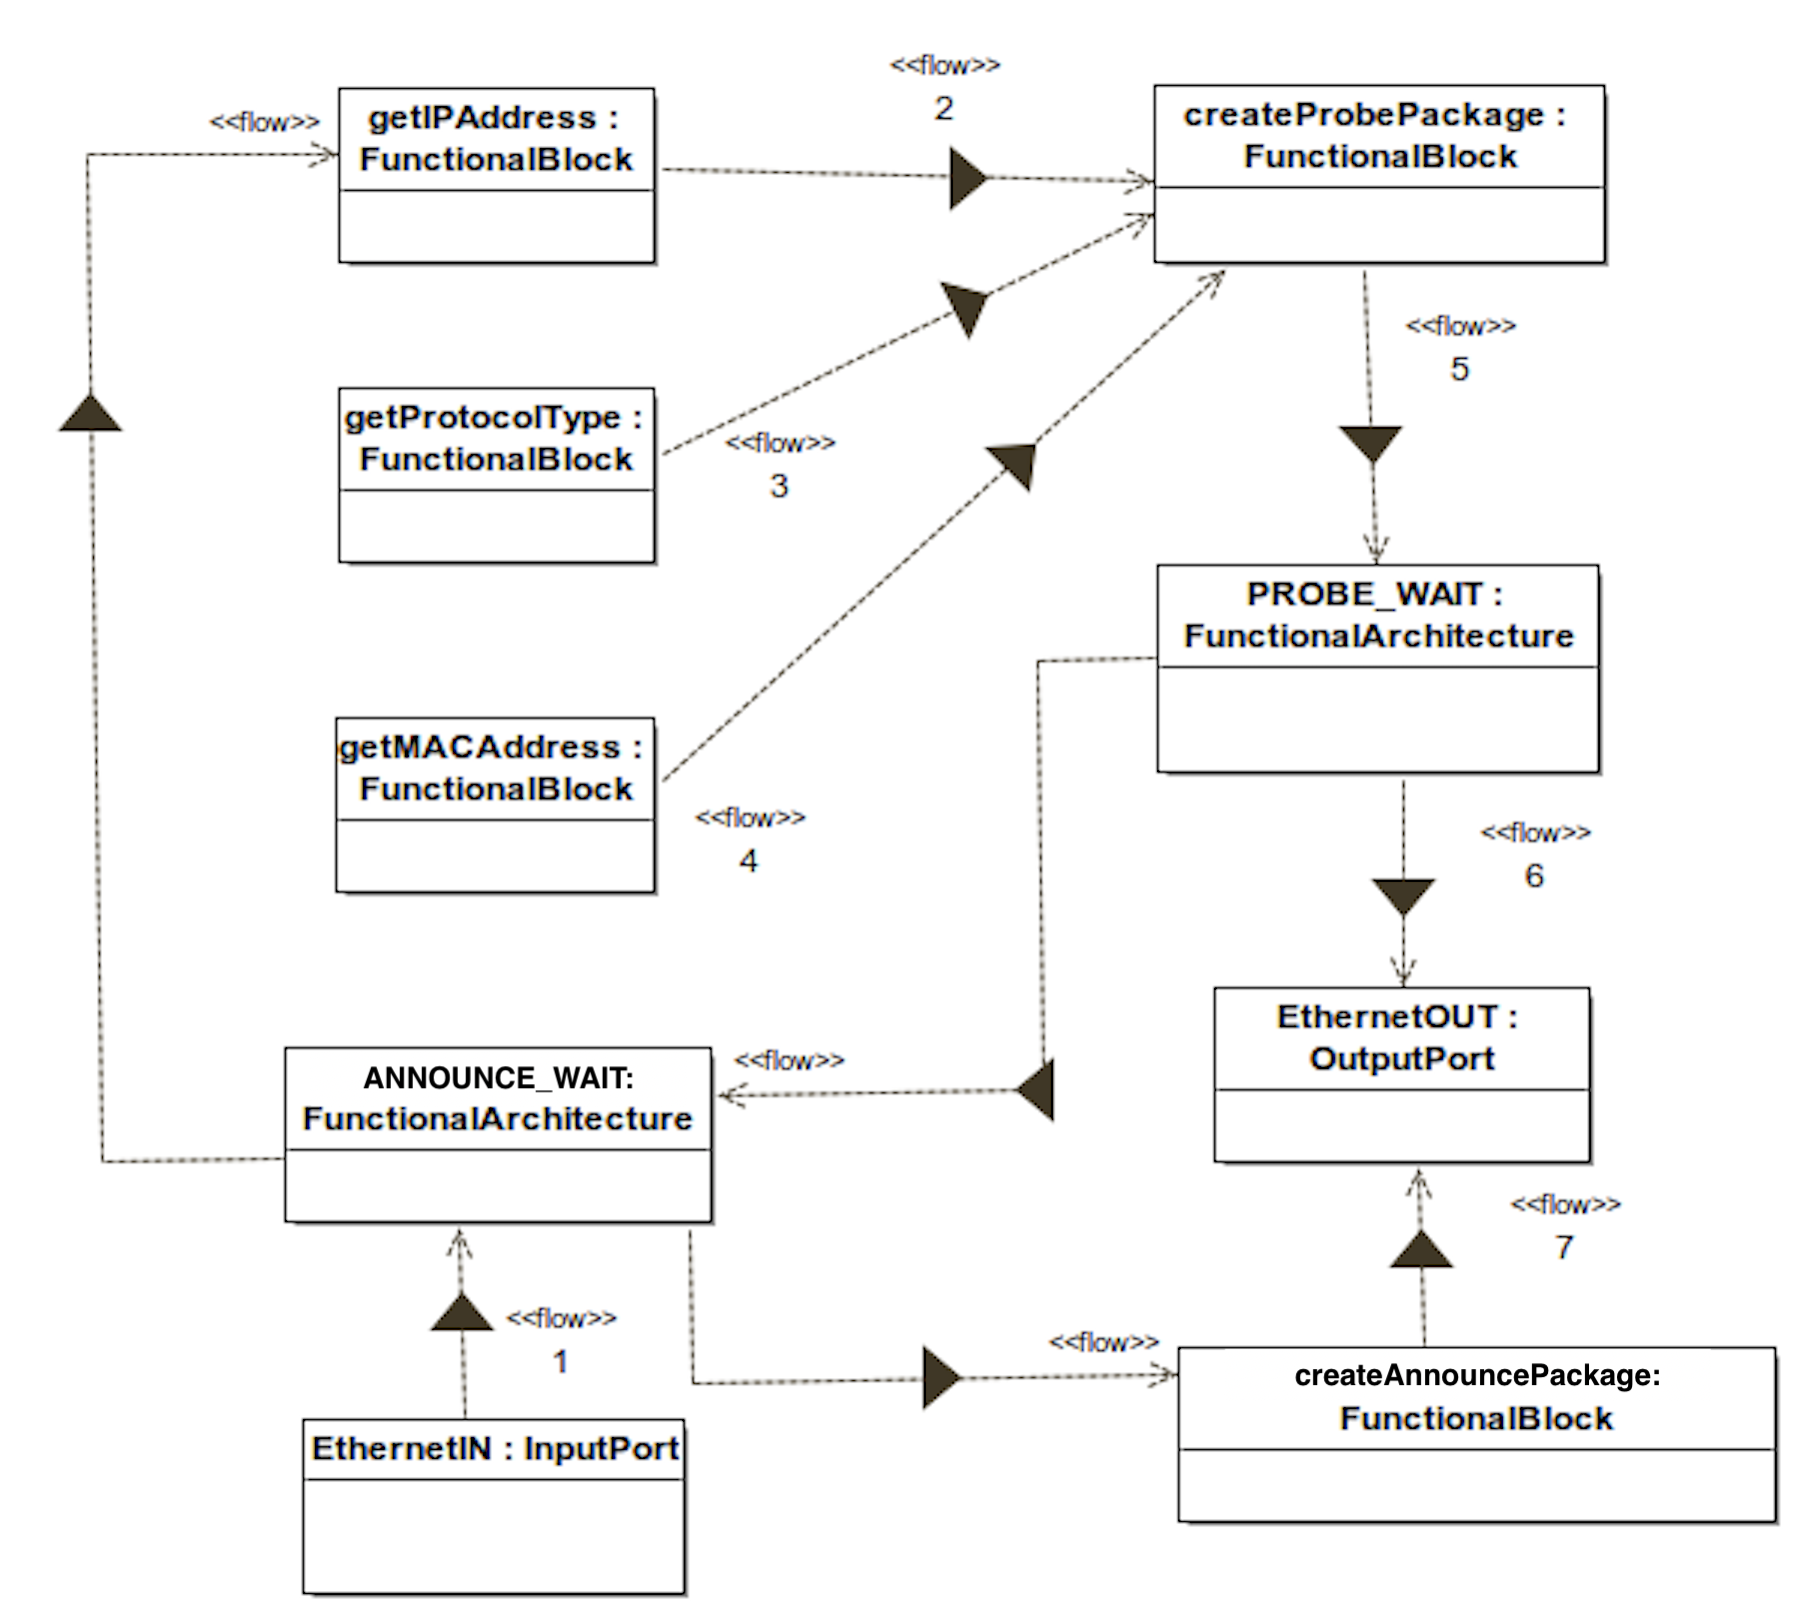
\includegraphics[scale=0.35]{../img/ARP/ARP.png}
    \begin{lstlisting}[frame=single, mathescape, basicstyle=\footnotesize]
1. $<\{as\$hrd, ar\$pro, ar\$hln, ar\$pln, reply, ar\$sha, ar\$spa, ar\$tha, ar\$tpa\}>$
2. $<ip>$
3. $<ar\$spa>$
4. $<ar\$sha>$
5. $<\{as\$hrd, ar\$pro, ar\$hln, ar\$pln, request, ar\$sha, 0.0.0.0, 00:00:00:00:00:00, ip\}>$
6. $<\{as\$hrd, ar\$pro, ar\$hln, ar\$pln, request, ar\$sha, 0.0.0.0, 00:00:00:00:00:00, ip\}>$
7. $<\{as\$hrd, ar\$pro, ar\$hln, ar\$pln, request, ar\$sha, ip, 00:00:00:00:00:00, ip\}>$
    \end{lstlisting}
    \caption{Modellazione del protocollo ARP} 
    \label{fig:ARP}
\end{figure}
\newpage
\begin{figure}[h!] 
    \centering 
    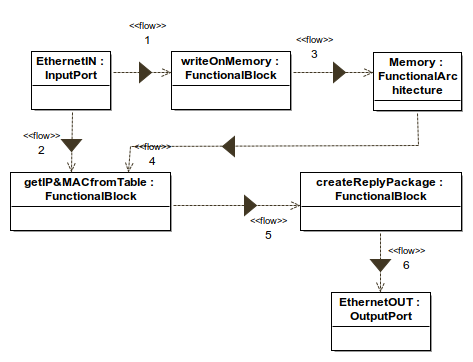
\includegraphics[scale=0.5]{../img/ARP/ARP_Reply_Object_diagram.png} 
\begin{lstlisting}[frame=single, mathescape, basicstyle=\footnotesize]
1. $<\{as\$hrd, ar\$pro, ar\$hln, ar\$pln, request, ar\$sha, ip, 00:00:00:00:00:00, ip\}>$
2. $<\{as\$hrd, ar\$pro, ar\$hln, ar\$pln, request, ar\$sha, 0.0.0.0, 00:00:00:00:00:00, ip\}>$
3. $<ar\$sha, ip>$
4. $<ar\$tha, ar\$tpa>$
5. $<ar\$tha, ar\$tpa>$
6. $<\{as\$hrd, ar\$pro, ar\$hln, ar\$pln, reply, ar\$sha, ar\$spa, ar\$tha, ar\$tpa\}>$
\end{lstlisting}
    \caption{Modellazione del blocco di ARP Reply} 
    \label{fig:ARP2}
\end{figure}
\noindent Nel caso in cui una macchina della rete riceva un pacchetto dall'oggetto EthernetIN (Figura \ref{fig:ARP2}), la prima cosa che fa è verificare se si tratta di un pacchetto di probe oppure di un pacchetto di announce.\\
Nel primo caso va a verificare con l'oggetto Memory se nell'ARP cache è già presente quell'indirizzo IP, assegnato ad un indirizzo MAC, che non corrisponde a quello del sender del pacchetto.\\ 
Se vi è una corrispondenza tra l'indirizzo ip del sender del pacchetto ed uno già presente nell'ARP cache, allora l'oggetto getIP\&MACFromTable riceve in input le informazioni dalla ARP cache per generare un nuovo pacchetto attraverso l'oggetto createReplyPackage, con il quale rispondere in unicast al sender attraverso l'oggetto EthernetOut, altrimenti non fa nulla.\\
Nel caso in cui si tratti di un pacchetto di announce allora l'oggetto writeOnMemory si occuperà di salvare nella ARP cache la mappatura tra l'indirizzo IP e MAC del sender.\\

\subsubsection*{Tool di verifica}
Dopo aver modellato il protocollo ed estratto il file .xmi visibile nel Listing \ref{lst:arp1}\footnote{\label{note:b}Listing in Appendice \ref{app:arp}}, si utilizza il tool di conversione per ottenere il file delle strutture Listing \ref{lst:arp2}\textsuperscript{\ref{note:b}}.\\
Per quanto già detto precedentemente, essendo il protocollo ARP suddivisibile in più scenari come l'invio del pacchetto di probe seguito dall'invio del pacchetto di announce oppure l'invio del pacchetto di probe seguito dall'invio del pacchetto di reply, una volta generato il template completo deve essere l'utilizzatore a suddividere i vari scenari per poi sottoporli alla verifica con Verifpal.\\
Per dividere i due scenari, l'utilizzatore deve generare due file da utilizzare come input in VerifPal, per fare questo è sufficiente copiare il template completo ed andare a cancellare le righe di generazione e invio del pacchetto di announce quando si vuole rappresentare lo scenario dell'invio del pacchetto di probe seguito dall'invio del pacchetto di reply, allo stesso modo per rappresentare lo scenario di invio di un pacchetto di probe seguito da un pacchetto di announce, l'utilizzatore non deve fare altro che cancellare le righe contenenti la creazione e l'invio del pacchetto di reply.
\newpage
\lstinputlisting[label={lst:arp_annunce.vp},caption={File arp\_announce.vp},language=vp, breaklines= true]{../code/verifpal/arp_annunce.vp}
\newpage
\lstinputlisting[label={lst:arp_reply.vp},caption={File arp\_reply.vp},language=vp, breaklines= true]{../code/verifpal/arp_reply.vp}

\noindent Come ben noto, il protocollo ARP è un protocollo di rete che non si occupa dell'integrità dei pacchetti ed è vulnerabile ad un attacco chiamato ARP Poisoning, questo attacco consiste in un attacco del tipo Man In The Middle, dove l'attaccante modifica i pacchetti che attraversano la rete per andare a modificare con valori inesatti le ARP cache delle macchine connesse.\\
L'obiettivo della modifica della mappatura tra indirizzo MAC e indirizzo IP può essere attuare un Denial Of Service oppure fingersi una determinata macchina.\\
Dato l'utilizzo dell'attaccante attivo da parte del tool VerifPal, come possiamo vedere dai Listing \ref{lst:arp3}-\ref{lst:arp4}\footnote{Listing in Appendice \ref{app:arp}}, l'attaccante riesce a violare sia la confidenzialità che l'integrità dei pacchetti, di conseguenza riesce ad attuare l'attacco di tipo ARP Poisoning.\\
Per confermare quanto appena detto in Appendice \ref{app:arp} vengono riportate la modellazione dello scenario di invio di un pacchetto di probe descritto in Applied Pi Calculus nel Listing \ref{lst:arp5} e il risultato della verifica svolta con ProVerif nel Listing \ref{lst:arp6}.\\ 
